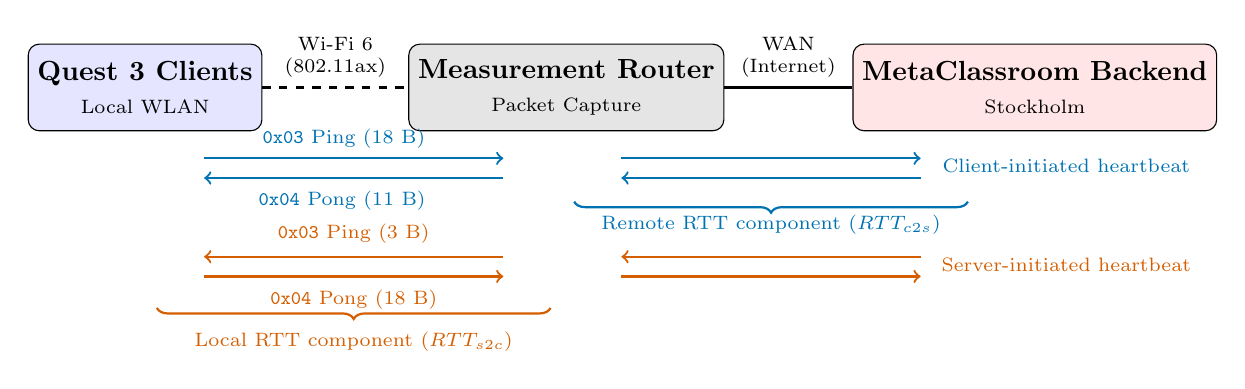
\begin{tikzpicture}
% Okabe-Ito colors matching Figures 2-4: client-initiated (c2s) = blue, server-initiated (s2c) = vermilion
\definecolor{cUp}{HTML}{0072B2}
\definecolor{cDown}{HTML}{D55E00}
% Boxes
\node[draw, rounded corners, minimum width=2.4cm, minimum height=1.1cm, fill=blue!10, align=center] (client) at (-1.15,0) {\textbf{Quest 3 Clients}\\\scriptsize Local WLAN}; \node[draw, rounded corners, minimum width=2.4cm, minimum height=1.1cm, fill=gray!20, align=center] (mid) at (4.2,0) {\textbf{Measurement Router}\\\scriptsize Packet Capture}; \node[draw, rounded corners, minimum width=2.4cm, minimum height=1.1cm, fill=red!10, align=center] (server) at (10.15,0) {\textbf{MetaClassroom Backend}\\\scriptsize Stockholm}; % Links 
\draw[thick,dashed] (client) -- node[midway,above, font=\scriptsize, align=center] {Wi-Fi 6\\(802.11ax)} (mid); \draw[thick] (mid) -- node[midway,above,font=\scriptsize, align=center] {WAN\\(Internet)} (server);
% -------------------------------------------------- % Client initiated heartbeat % -------------------------------------------------- 
\node[font=\scriptsize, text=cUp] at (10.55,-1) {Client-initiated heartbeat}; % Ping: Client -> Server 
\draw[->,thick,cUp] (-0.4,-0.9) -- node[midway,above,font=\scriptsize,pos=0.467201] {\texttt{0x03} Ping (18 B)} (3.4,-0.9); \draw[->,thick,cUp] (4.9,-0.9) -- (8.7,-0.9); % Pong: Server -> Client 
\draw[<-,thick,cUp] (-0.4,-1.15) -- (3.4,-1.15); \draw[<-,thick,cUp] (4.9,-1.15) -- node[midway,below=1pt,font=\scriptsize,pos=-0.933378] {\texttt{0x04} Pong (11 B)} (8.7,-1.15); % RTT brace 
\draw[ decorate, decoration={brace,mirror,amplitude=4pt}, thick, cUp ] (4.3,-1.45) -- (9.3,-1.45) node[midway,below=1pt,font=\scriptsize] {Remote RTT component ($RTT_{c2s}$)}; % -------------------------------------------------- % Server initiated heartbeat % -------------------------------------------------- 
\node[font=\scriptsize, text=cDown] at (10.55,-2.25) {Server-initiated heartbeat}; % Ping: Server -> Client 
\draw[<-,thick,cDown] (-0.4,-2.15) -- node[midway,above=1pt,font=\scriptsize,pos=0.50] {\texttt{0x03} Ping (3 B)} (3.4,-2.15); \draw[<-,thick,cDown] (4.9,-2.15) -- (8.7,-2.15); % Pong: Client -> Server 
\draw[->,thick,cDown] (-0.4,-2.4) -- node[midway,below=1pt,font=\scriptsize,pos=0.50] {\texttt{0x04} Pong (18 B)} (3.4,-2.4); \draw[->,thick,cDown] (4.9,-2.4) -- (8.7,-2.4); % RTT brace 
\draw[ decorate, decoration={brace,mirror,amplitude=4pt}, thick, cDown ] (-1,-2.8) -- (4,-2.8) node[midway,below=5pt,font=\scriptsize] {Local RTT component ($RTT_{s2c}$)};
\end{tikzpicture}